%! TEX rootmain.tex

\chapter{Violin}

The violin is a bowed-string instrument in which sustained excitation is provided by frictional interaction between bow and strings. The string motion is transmitted to the body through the bridge, and the vibrating structure radiates sound through a combination of structural and air-coupled mechanisms. Following the course outline, the discussion starts from the instrument anatomy and then moves to historical notes, bowed-string motion, body vibrations and transient response, internal components such as soundpost and bass bar, the bridge and its coupling to the soundboard, sound radiation, wolf notes, and electrical analog models.

\section{Anatomy of the Violin}

A reference view of the violin and its main components is shown in figure \ref{fig:violin_anatomy}.

\begin{figure}[!htb]
\centering
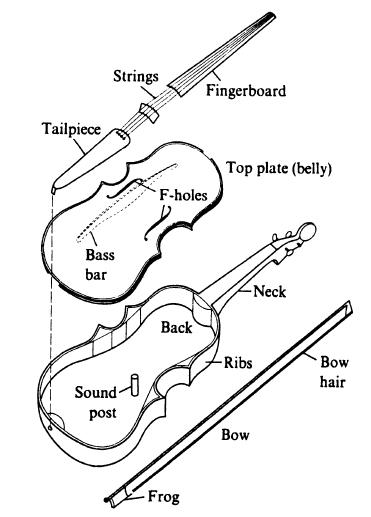
\includegraphics[width=0.6\linewidth]{00_Images/03_chapter/img53.jpg}
\caption{Anatomy of the violin and main components}
\label{fig:violin_anatomy}
\end{figure}

\subsection{Main Components and Materials}

A violin can be described by its strings, the carved wooden body, and a small set of internal components that strongly influence vibration transfer. The strings are typically steel, gut, or nylon, tuned to \( G_3 \), \( D_4 \), \( A_4 \), and \( E_5 \). The top plate is commonly carved from spruce, such as Picea abies or Picea excelsis, while back, ribs, and neck are commonly made from maple, such as Acer platanoides. The fingerboard is made from ebony and the bow stick from Pernambuco. Under the top plate, the bass bar provides local stiffening. The soundpost is positioned near the treble foot of the bridge and provides a mechanical coupling between top and back plates. 

\subsection{Geometry, Thicknesses, and Static Loads}

Typical violin dimensions are about \SI{35}{\centi\meter} in body length, with upper and lower bout widths of about \SIrange{16}{20}{\centi\meter}. Ribs are about \SIrange{30}{32}{\milli\meter} high. Plate thickness varies across the instrument. Representative values are \SIrange{2.0}{3.5}{\milli\meter} for the top plate and \SIrange{2.0}{6.0}{\milli\meter} for the back, while the maximum arch height of both plates is about \SI{15}{\milli\meter}. Exact thickness and arching depend on the violin-maker choices and on the vibroacoustic behavior of the specific wood piece. On the top plate, a channel is cut along the edge and filled with strips of wood called purfling. This detail promotes a boundary behavior closer to hinged than clamped, allowing larger plate mobility near the edge. The total string tension is about \SI{220}{\newton}. The resulting downward force on the bridge is about \SI{90}{\newton}, supported by the arching and internally by the bass bar and the soundpost.

\subsection{Sound Production in Brief}

Sound production can be summarized as a short chain of coupled events:

\begin{itemize}
    \item The violinist draws the bow across the strings, setting them into vibration.
    \item The vibrating strings exert forces on the bridge and excite the body motion.
    \item The body vibration produces acoustic radiation.
\end{itemize}

While the sequence appears simple, many subtleties are hidden in the excitation and in the coupled structural response, which is why the violin is among the most studied musical instruments. 

\section{Motion of Bowed Strings}

In bowed-string excitation, the frictional interaction between bow and string produces a stick-slip motion that generates one or more traveling bends. These bends run around a curved envelope, whose maximum amplitude depends on the bow speed and on the bowing position. Bowing at a single point divides the string into two segments. The basic kinematics of bowed-string motion, including sticking and slipping phases, is summarized in figure \ref{fig:bowed_string_motion_basic}.

\begin{figure}[!htb]
\centering
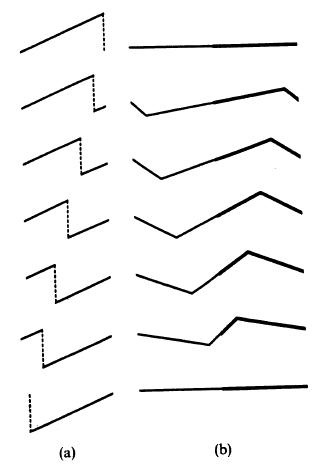
\includegraphics[width=0.6\linewidth]{00_Images/03_chapter/img80.jpg}
\caption{Basic description of bowed-string motion over a cycle}
\label{fig:bowed_string_motion_basic}
\end{figure}

If \( x_b \) is the distance from the bridge to the bowing point and \( L \) is the string length, the segment lengths are in the ratio
\[
\frac{L-x_b}{x_b} = p
\]
The resulting velocity pattern can be interpreted as the superposition of a positive and a negative traveling wave of the same form. When the two waves are coincident, the velocity diagram becomes a straight line passing through one end of the string, with a discontinuity at the other. A modal representation of the transverse displacement is
\[
y(x,t) = \sum_{n = 1}^{\infty} a_n \sin\left(\frac{n\pi x}{L}\right)\sin(n\omega t)
\]
In inappropriate bowing conditions, in particular when the bowing force is not sufficient in relation to the bowing position, more than a single bend can be generated. This may lead to double-slip or multiple-flyback regimes, producing force waveforms at the bridge that differ markedly from the regular Helmholtz motion. Examples of non-ideal periodic regimes such as double-slip and multiple-flyback motion are shown in figure \ref{fig:bowed_string_nonideal}.

\begin{figure}[!htb]
\centering
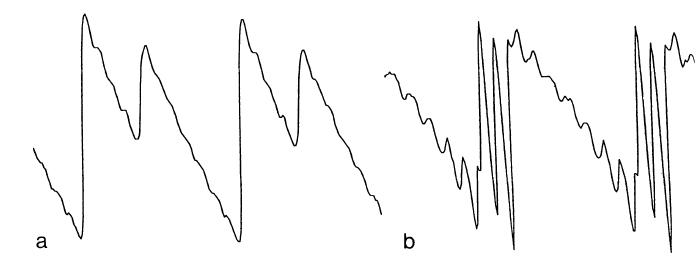
\includegraphics[width=0.7\linewidth]{00_Images/03_chapter/img105.jpg}
\caption{Non-ideal bowed-string regimes: double slip and multiple flyback}
\label{fig:bowed_string_nonideal}
\end{figure}

Louder playing requires both higher bow speed and bowing closer to the bridge. A compact estimate links these parameters to the maximum displacement and to the maximum transverse force at the bridge,
\[
y_m = \frac{1}{8f}\frac{v_b}{x_b}
\]
\[
F_m = \mu c \frac{v_b}{x_b}
\]
where \( v_b \) is the bowing speed, \( f \) is the playing frequency, \( \mu \) is the string mass per unit length, and \( c \) is the transverse wave speed. Due to string stiffness, the Helmholtz corner is not perfectly sharp. Two consequences are commonly observed: the pitch can flatten as bow force increases, and the period can show jitter, with variations up to about \SI{30}{cent} between minimum and maximum values. Besides transverse motion, bowed strings can support additional wave types. Longitudinal vibrations generate sounds that are not harmonically related to the transverse partials. Representative longitudinal-mode frequencies are around \SI{1350}{\hertz} and \SI{2700}{\hertz} for the \( G \) and \( D \) strings. Torsional waves are also excited by the bowing action, with propagation speed
\[
c_T = \sqrt{\frac{G K_T}{\rho I}}
\]
where \( G \) is the shear modulus, \( K_T \) is a torsional stiffness factor, \( \rho \) is the density, and \( I \) is the polar moment of inertia. The ratio between torsional and longitudinal wave speeds is
\[
\frac{c_T}{c_L} = \frac{1}{\sqrt{2(1+\nu)}}
\]
It typically ranges from about \( 1/7.7 \) to \( 1/2 \), depending on the material, and torsional damping is usually much higher than transverse damping. The bow hair alone does not provide sufficient friction to trigger a stable stick-slip regime, so rosin plays a central role. Rubbing the bow with rosin deposits fragments of various sizes: larger ones tend to detach after a few strokes, while smaller ones adhere more firmly. During playing, rosin warms up, its static friction coefficient increases, and its sliding coefficient decreases. As a consequence, during slip the rosin tends to act as a lubricant, while during stick it increases bow-string friction and promotes a longer stick phase. A typical velocity-dependent friction characteristic used in dynamic bowing models is shown in figure \ref{fig:bow_friction_characteristic}.

\begin{figure}[!htb]
\centering
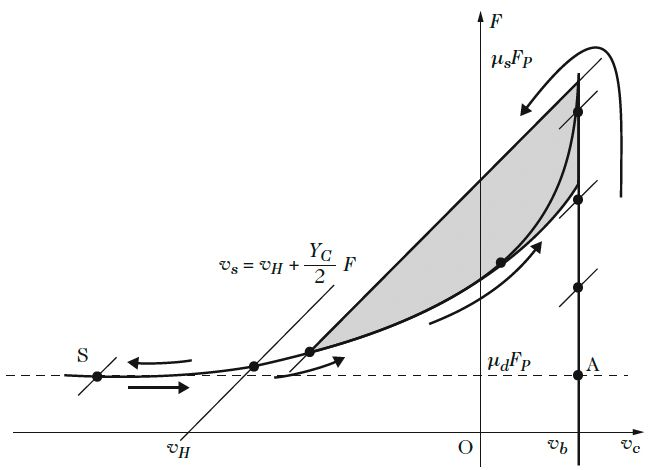
\includegraphics[width=0.7\linewidth]{00_Images/03_chapter/img127.jpg}
\caption{Velocity-dependent friction characteristic for bow-string interaction}
\label{fig:bow_friction_characteristic}
\end{figure}

\subsection{Dynamic Model}

A compact dynamic model can be written in terms of the string velocity at the bowing point \( v_s(t) \), the bow velocity \( v_b \) (assumed constant during the observation window), and the bow-string interaction force \( F(t) \),
\[
v_s(t) = \left[F \star v_{\delta}\right](t)
\]
\[
F(t) = F_{NL}\!\left[v_s(t) - v_b\right]
\]
where \( v_{\delta}(t) \) is the string velocity response to an impulsive force at the bowing point and \( F_{NL} \) is the friction curve as a function of relative velocity. It is useful to decompose the velocity as
\[
v_s(t) = v_h(t) + v_{\infty,\infty}(t)
\]
where \( v_h(t) \) is due to the history of traveling waves on the finite string and \( v_{\infty,\infty}(t) \) is due to the instantaneous action of the bow, obtained by assuming the string infinite in both directions. Introducing the characteristic admittance \( Y_c \) of an equivalent infinite string, one obtains
\[
v_{\infty,\infty}(t) = \frac{Y_c}{2}F(t)
\]
The friction law must account for different static and dynamic friction coefficients, with \( \mu_s>\mu_d \). Representative values may be \( \mu_s = 0.7 \) and \( \mu_d = 0.2 \), and experiments indicate a transition region between the two regimes. In the \( (v_s,F) \) plane, the system state is found as the intersection between the straight line
\[
v_s(t) = v_h(t) + \frac{Y_c}{2}F(t)
\]
and the friction curve. When the pressing force is small enough, the slope of the friction curve remains below \( 2/Y_c \) and only one intersection exists. When the pressing force exceeds a threshold, \( 2/Y_c \) becomes smaller than the steepest slope of the friction curve and two intersections may appear, corresponding to a sticking point and a sliding point, with the force at the sticking point larger than at the sliding point.

\subsection{Schelleng's Diagram}

For each bowing position there exists a minimum and a maximum bowing force for which the bend can trigger the beginning and end of slippage between bow and string. This is summarized by Schelleng's diagram, which provides the admissible range of bow forces as a function of the bow-to-bridge distance. As the bowing point approaches the bridge, the distance between the minimum and maximum admissible forces becomes smaller. Bowing closer to the bridge therefore requires a considerably larger and more precisely controlled force, while also leaving a reduced margin before irregular regimes such as multiple slips occur. The admissible bowing range in terms of bow force and distance from the bridge is summarized by Schelleng's diagram in figure \ref{fig:schelleng_diagram}.

\begin{figure}[!htb]
\centering
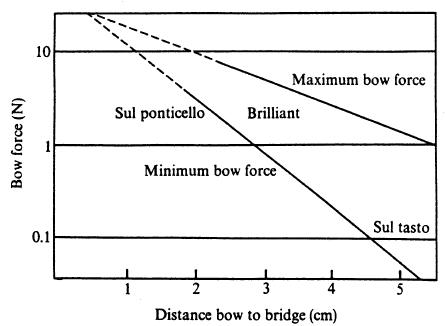
\includegraphics[width=0.7\linewidth]{00_Images/03_chapter/img144.jpg}
\caption{Schelleng's diagram for bowing limits}
\label{fig:schelleng_diagram}
\end{figure}

The combined transverse and torsional components of bowed-string motion can be visualized as in figure \ref{fig:lissajous_torsion_helmholtz}.

\begin{figure}[!htb]
\centering
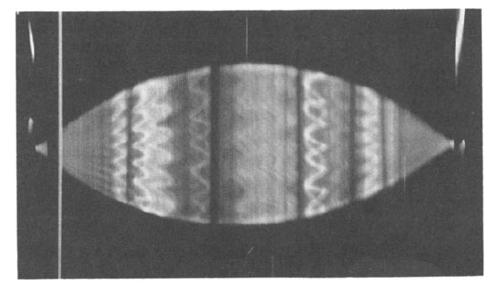
\includegraphics[width=0.7\linewidth]{00_Images/03_chapter/img159.jpg}
\caption{Lissajous representation highlighting torsional and Helmholtz components}
\label{fig:lissajous_torsion_helmholtz}
\end{figure}

\section{Violin Body Vibrations}

Violin vibrations are mainly due to the coupled motions of the top and back plates and to the enclosed air. Motions of fingerboard and ribs may be present, but they are not considered acoustically relevant in a first approximation. For modeling purposes, low-frequency behavior can be represented by a network analog, but this becomes rapidly complex because of the coupling introduced by the soundpost. For this reason, finite element modeling is often adopted to describe the vibrational response over a wider frequency range. A comparison of bridge admittance measured on different violins shows that modal frequencies vary from one instrument to another, while the overall admittance trend remains qualitatively similar. This shared trend is one of the features that makes different instruments recognizable as violins. Measured bridge admittance curves for different violins are compared in figure \ref{fig:bridge_admittance_multiple_violins}.

\begin{figure}[!htb]
\centering
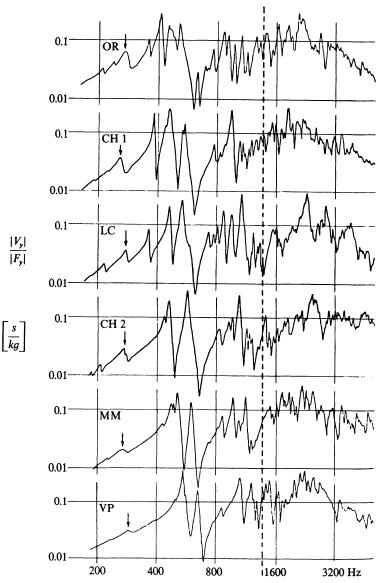
\includegraphics[width=0.5\linewidth]{00_Images/03_chapter/img174.jpg}
\caption{Bridge admittance measured on several violins}
\label{fig:bridge_admittance_multiple_violins}
\end{figure}

Even when resonance frequencies shift, modes can still be categorized according to their deformation shapes, which are comparatively invariant. Different nomenclatures exist for violin modes. In the following, mode labels are reported as \( \text{Name 1 [Name 2]} \), where the two names refer to two commonly used naming conventions.

\paragraph{Low-frequency bending modes} The mode \( C1[B^-] \) is a one-dimensional bending resembling the first bending mode of a bar. It features one nodal line near the bridge and another about halfway toward the neck, and it occurs on average around \SI{185}{\hertz}. A second bending mode (not shown) is sometimes denoted \( N \) and involves motion of neck and fingerboard. These bending-type modes are not associated with strong radiation. The first mode of major acoustical importance is the f-hole resonance \( A0[A0] \), in which a substantial amount of air moves in and out of the f-holes. It is often referred to as a Helmholtz resonance, with the caveat that the violin walls are not rigid. Its frequency is on average around \SI{275}{\hertz}. A two-dimensional flexural mode \( C2 \) is typically observed around \SI{405}{\hertz}. The mode \( T1[B1^-] \) is mainly a motion of the top plate, with average frequency around \SI{460}{\hertz}. The mode \( C3[B1^+] \) is a two-dimensional motion involving both plates and is typically around \SI{530}{\hertz}. Another important two-dimensional mode \( C4 \) occurs around \SI{700}{\hertz}. Among these, the modes designated \( A0 \), \( T1 \), \( C3 \), and \( C4 \) are often treated as the most relevant in the low-frequency range. Instruments judged best in quality tend to show a uniformly high admittance level associated with these modes. In addition, the increase in admittance between about \SIrange{1.4}{3}{\kilo\hertz}, known as the bridge hill, is commonly regarded as an important quality factor. The main low-frequency body modes (often referred to as signature modes) are illustrated in figure \ref{fig:violin_signature_modes}.

\begin{figure}[!htb]
\centering
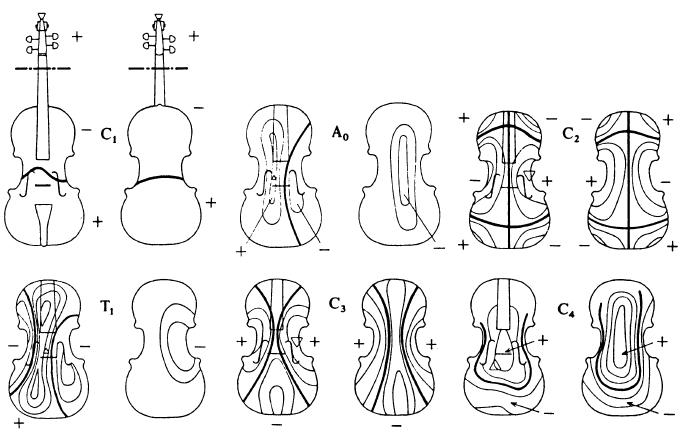
\includegraphics[width=0.7\linewidth]{00_Images/03_chapter/img189.jpg}
\caption{Representative violin body modes at low frequency}
\label{fig:violin_signature_modes}
\end{figure}

\paragraph{Component analysis in lutherie} In practical making and setup, it is useful to analyze the vibrational modes of different components separately, to obtain hints on the assembled outcome. Air modes can be estimated by building rigid-wall cavities with violin-like shape, by immersing the instrument in sand, or by finite element analysis, with results that are generally in good agreement. A schematic view related to cavity (air) modes and their identification is shown in figure \ref{fig:violin_air_modes}.

\begin{figure}[!htb]
\centering
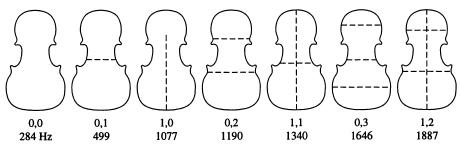
\includegraphics[width=0.7\linewidth]{00_Images/03_chapter/img206.jpg}
\caption{Illustration related to violin cavity (air) modes}
\label{fig:violin_air_modes}
\end{figure}

\paragraph{Free plates and assembled body} The modal frequencies of free plates are not directly related to those of the assembled body, because complex coupling arises when plates are mounted together with back and ribs. Tuning selected free-plate modes, such as the X-mode (mode \#2) and the ring mode (mode \#5), approximately one octave apart in the two plates are proposed by some studies. Given the X-mode frequencies, it has been suggested that the intended use of the instrument can be anticipated. For cellos, mode \#1 can be tuned about one octave below mode \#2 in both plates, while in violins the corresponding interval should be less than an octave in the back plate. Examples of free-plate mode shapes (often visualized via Chladni patterns) are shown in figure \ref{fig:free_plate_modes_chladni}.

\begin{figure}[!htb]
\centering
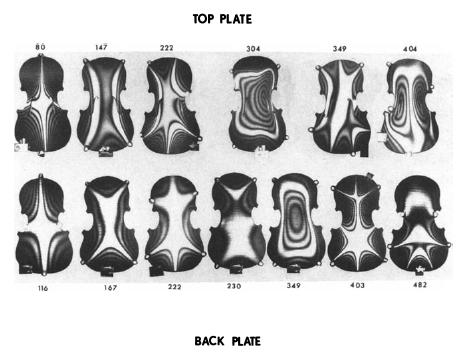
\includegraphics[width=0.7\linewidth]{00_Images/03_chapter/img220.jpg}
\caption{Free-plate mode shapes for top and back plates}
\label{fig:free_plate_modes_chladni}
\end{figure}

\section{Transient Wave Response of the Violin Body}

\subsection{Impulse Excitation at the Bridge}

Besides steady-state admittance and modal shapes, it is important to study the short-time response of the violin body to impulsive forces applied at the bridge. In particular, both transversal and longitudinal impulsive excitations are relevant, because they correspond to different directions of the string-bridge interaction and they trigger different wave-like motions in the plates. Transient wave propagation following impulsive excitation is illustrated by interferograms in figure \ref{fig:violin_transient_interferograms}.

\begin{figure}[!htb]
\centering
\subfloat{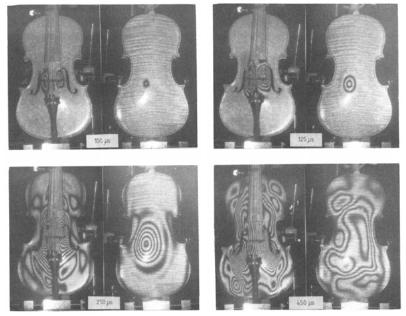
\includegraphics[height=0.3\textheight]{00_Images/03_chapter/img236.jpg}}\hfill
\subfloat{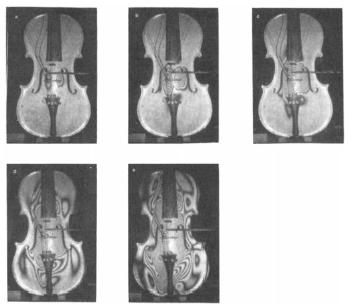
\includegraphics[height=0.3\textheight]{00_Images/03_chapter/img250.jpg}}
\caption{Interferograms after impulsive excitation in two directions}
\label{fig:violin_transient_interferograms}
\end{figure}

\subsection{Impulse Parallel to the Top Plate}

When an impulsive force is applied parallel to the top plate at the bridge, interferograms of top and back plates show the development of transient deformation patterns on microsecond time scales. Representative snapshots reported at \( t = \SI{100}{\micro\second} \), \( \SI{125}{\micro\second} \), \( \SI{250}{\micro\second} \), and \( \SI{450}{\micro\second} \) highlight how the disturbance propagates away from the bridge region and excites coupled motion of both plates. 

\subsection{Impulse Orthogonal to the Top Plate}

If the impulsive force is orthogonal to the top plate, the transient response differs markedly. Interferograms at \( t = \SI{70}{\micro\second} \), \( \SI{120}{\micro\second} \), \( \SI{150}{\micro\second} \), \( \SI{230}{\micro\second} \), and \( \SI{300}{\micro\second} \) show patterns that are distinct from the parallel-force case, indicating that the initial loading direction selects different families of plate motion and coupling mechanisms. 

\subsection{Phase Relation Between Bridge Feet}

A key qualitative difference between the two excitations concerns the phase relation of the impulses transmitted through the bridge feet.

\begin{itemize}
    \item For a force parallel to the plate, the pulses transmitted to the treble and bass feet are equal in magnitude but opposite in phase.
    \item For a transversal input, the original pulses have the same phase on the two sides of the bridge.
\end{itemize}

This difference explains why the observed interferometric patterns for the two loading directions are not simply scaled versions of each other, but instead exhibit different spatial organizations from the earliest instants after the impulse. 

\section{Soundpost and Bass Bar}

The vibroacoustic behavior of the violin body is rendered asymmetrical by the presence of the soundpost and the bass bar, located approximately beneath the treble and bass feet of the bridge, respectively. Strings are excited mainly parallel to the top plate, thus inducing a rocking motion of the bridge. Below the first resonance of the bridge, typically around \SI{2500}{\hertz} for a violin, the forces exerted on the two bridge feet are approximately equal in magnitude and opposite in phase. In a perfectly symmetric instrument, such a loading would preferentially excite only antisymmetric body modes, while strongly radiating symmetric modes would be driven only weakly. In practice, the asymmetry introduced by soundpost and bass bar alters this selection mechanism and contributes to the excitation of efficiently radiating motions. 

\subsection{Role of the Bass Bar}

The main function of the bass bar is to stiffen the top plate, both statically and dynamically. In many valuable historical instruments the bass bar has been modified over time, because modern strings exert higher tension than in the past and a stiffer support of the top plate becomes necessary.

\subsection{Role of the Soundpost} 

The soundpost mechanically couples the top and back plates. To clarify its effect, several investigators have compared violins with and without a soundpost. One reported set of observations found that removing the soundpost produced the following changes: 

\begin{itemize}
    \item It lowered the frequencies of the \( A0 \) and \( T1[B1] \) modes by \( 8\% \) and \( 13\% \), respectively.
    \item It made the \( T1 \) mode comparatively more symmetric.
    \item It raised the frequency of the \( C3 \) mode by about \( 2\% \).
    \item It left the \( A1 \) internal air mode essentially unchanged.
    \item It introduced a \( T2 \) mode, consisting largely of antisymmetric bending of the top plate.
\end{itemize}

As a consequence, in the presence of the soundpost, the strongly radiating \( T1 \) mode can be interpreted as a combination of a symmetric \( T1 \)-type motion and an antisymmetric \( T2 \)-type contribution. Another study suggests that removing the soundpost may leave the frequencies of \( T1 \) and \( C3 \) virtually unchanged while significantly modifying the corresponding mode shapes, with a dramatic decrease in radiation efficiency (estimated from measured mode shapes via boundary element methods) in the \SIrange{500}{800}{\hertz} range. These results are consistent with practical experience: violin makers and performers observe that moving the soundpost by a small distance can cause marked changes in the perceived sound of the instrument. 

\section{The Bridge}

The bridge transforms the motion of the vibrating strings into periodic driving forces applied to its feet and then to the top plate. Because it sits at the main mechanical interface between strings and body, any modification to the bridge can alter the instrument response and, consequently, the perceived sound. A convenient frequency-domain description uses the input impedance at the string notch and the force transfer from the notch to the two feet. If \( F_{\mathrm{in}}(\omega) \) and \( V_{\mathrm{in}}(\omega) \) are the force and velocity at the notch, and \( F_i(\omega) \) is the force delivered to foot \( i \), one may write
\[
Z_{\mathrm{in}}(\omega) = \frac{F_{\mathrm{in}}(\omega)}{V_{\mathrm{in}}(\omega)}, \quad H_i(\omega) = \frac{F_i(\omega)}{F_{\mathrm{in}}(\omega)}
\]
Measured curves show that the transfer to the two feet is not identical: the foot on the soundpost side and the foot on the bass bar side can exhibit different resonant features, reflecting the asymmetry of the coupled bridge-body system. The bridge mechanical response, including input impedance and force transfer, is shown in figure \ref{fig:bridge_impedance_force_transfer}.

\begin{figure}[!htb]
\centering
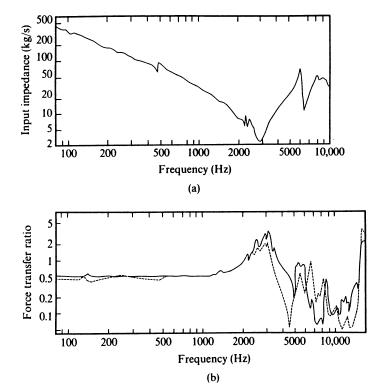
\includegraphics[width=0.7\linewidth]{00_Images/03_chapter/img267.jpg}
\caption{Bridge response: input impedance and force transfer ratio versus frequency}
\label{fig:bridge_impedance_force_transfer}
\end{figure}

\paragraph{First bridge resonances and mode shapes} The first two vibrational modes of a violin bridge occur in the kilohertz range and have distinct deformation patterns. The first resonance is mainly a rotation of the upper part of the bridge, while the second mode is efficiently excited by a vertical force. A comparison with a cello bridge highlights a different behavior: in the cello, the first modes are more strongly related to bending of the legs. This is attributed to the different bridge shape, characterized by more slender legs than the violin bridge. The first bridge modes and a comparison between violin and cello bridges are shown in figure \ref{fig:bridge_modes_violin_cello}.

\begin{figure}[!htb]
\centering
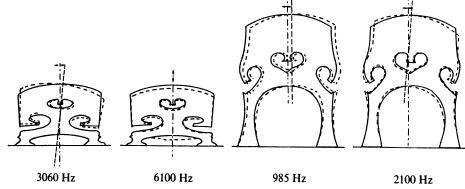
\includegraphics[width=0.7\linewidth]{00_Images/03_chapter/img281.jpg}
\caption{First bridge modes: comparison between violin and cello bridges}
\label{fig:bridge_modes_violin_cello}
\end{figure}

\paragraph{Practical modifications: added mass and added stiffness} Sometimes players modify the bridge response using simple interventions:

\begin{itemize}
    \item A mute, which acts mainly as a small added mass, tends to darken the sound by shifting bridge resonances toward lower frequencies.
    \item Small wedges pushed into bridge slits increase local stiffness and tend to raise modal frequencies.
\end{itemize}

A reported comparison of force transfer functions shows how an additional mass of about \SI{1.5}{\gram} and additional stiffness produce distinct shifts of the bridge resonances, confirming that relatively small changes at the bridge can have audible consequences. The effect of adding mass or stiffness to the bridge on force transfer is shown in figure \ref{fig:bridge_modifications_effect}.

\begin{figure}[!htb]
\centering
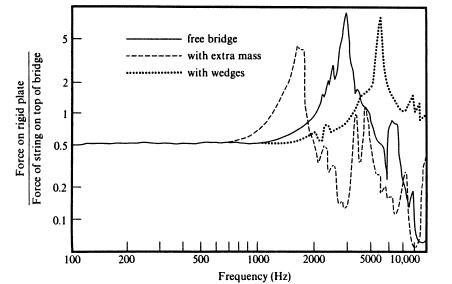
\includegraphics[width=0.7\linewidth]{00_Images/03_chapter/img295.jpg}
\caption{Effect of added mass and stiffness on bridge force transfer}
\label{fig:bridge_modifications_effect}
\end{figure}

\section{Coupling Between Bridge and Soundboard}

\subsection{Filtering Effect and Simplified Translation Model}

The coupling between bridge and soundboard can be described in terms of the input admittance seen by the strings at the bridge. Even a very simple coupled model already highlights an important consequence: the bridge does not transmit string forces uniformly with frequency, but introduces a filtering effect that shapes the response. A schematic model for the coupling between bridge motion and soundboard dynamics is shown in figure \ref{fig:bridge_soundboard_coupling_model}. A first approximation models the bridge as a lumped mass-spring system \( (m,k) \) loaded by the board admittance \( Y(\omega) \) at the attachment point. Denoting by \( V_b \) the bridge velocity at the string junction and by \( V_t \) the velocity of the board translation, the equations of motion are
\[
\begin{aligned}
&-m\omega^{2}V_b + k(V_b - V_t) = j\omega F \\
&V_t = Y(\omega)F_t = \frac{kY(\omega)}{j\omega}(V_b - V_t)
\end{aligned}
\]
The input admittance at the bridge is defined as
\[
Y_b(\omega) = \frac{V_b}{F}
\]
and it can be written as
\[
Y_b(\omega) = \frac{kY(\omega)+j\omega}{k-m\omega^{2}+j\omega k m Y(\omega)}
\]
If the bridge base is fixed, \( Y(\omega) = 0 \), the system reduces to a series resonance corresponding to the bridge eigenmode. In all other cases, the input admittance depends on the board mobility \( Y(\omega) \) and the resulting modulus \( |Y_b| \) can exhibit a pronounced peak in the kilohertz range, consistent with the bridge-hill feature observed in violin measurements.

\begin{figure}[!htb]
\centering
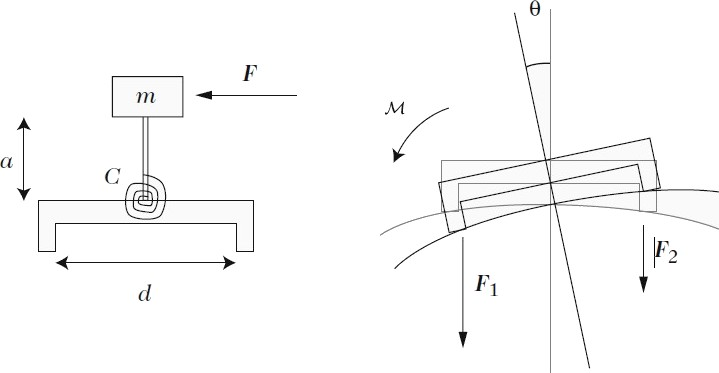
\includegraphics[width=0.7\linewidth]{00_Images/03_chapter/img385.jpg}
\caption{Model of coupling between bridge and soundboard}
\label{fig:bridge_soundboard_coupling_model}
\end{figure}

\subsection{Refined Model Including Bridge Rotation}

The previous model captures the existence of a bridge-related filtering peak, but it does not include any bridge geometry. A more realistic description accounts for the bridge rotation driven by the horizontal string force. Let the string apply a horizontal force \( F \) at a mean lever arm \( a \), generating a moment
\[
M = Fa
\]
The bridge rotation \( \theta \) is described by a torsional stiffness \( C \) and an effective rotational inertia \( ma^{2} \), so that
\[
M = ma^{2}\ddot{\theta}+C\theta
\]
and the corresponding angular eigenfrequency is
\[
\omega_b = \sqrt{\frac{C}{ma^{2}}}
\]
The bridge is connected to the soundboard through two feet separated by a distance \( d \). Under the forces \( (F_1,F_2) \), the foot velocities \( (V_1,V_2) \) satisfy an admittance-matrix relation
\[
\begin{bmatrix}
V_1 \\
V_2
\end{bmatrix}
 = 
\begin{bmatrix}
Y_{11} & Y_{12} \\
Y_{21} & Y_{22}
\end{bmatrix}
\begin{bmatrix}
F_1 \\
F_2
\end{bmatrix}
\]
With one foot fixed, a moment \( M \) can be represented by the equivalent force couple
\[
F_1 = \frac{M}{d^{2}}, \quad F_2 = -\frac{M}{d^{2}}
\]
leading to
\[
\begin{bmatrix}
\dot{\theta}_1 \\
\dot{\theta}_2
\end{bmatrix}
 = 
\begin{bmatrix}
Y_{11} & Y_{12} \\
Y_{21} & Y_{22}
\end{bmatrix}
\begin{bmatrix}
\dfrac{M}{d^{2}} \\
-\dfrac{M}{d^{2}}
\end{bmatrix}
\]
The bridge rotational velocity is \( \dot{\theta} = \dot{\theta}_1-\dot{\theta}_2 \), hence the rotational admittance is
\[
Y_r(\omega) = \frac{\dot{\theta}}{M} = \frac{Y_{11}+Y_{22}-2Y_{12}}{d^{2}}
\]

\subsection{Rotational Admittance in Modal Form and Bridge Input Admittance}

The rotational admittance can be expressed in modal form in terms of soundboard eigenshapes \( \phi_n \), evaluated at the two foot locations \( (x_1,y_1) \) and \( (x_2,y_2) \),
\[
Y_r(\omega) = j\omega\frac{1}{d^{2}}
\sum_{n}
\frac{\left[\phi_n(x_1,y_1)-\phi_n(x_2,y_2)\right]^{2}}
{m_n\left(\omega_n^{2}+2j\omega\omega_n\zeta_n-\omega^{2}\right)}
\]
where \( m_n \) is the modal mass, \( \omega_n \) the eigenfrequency, and \( \zeta_n \) the modal damping ratio. Finally, the bridge input admittance follows by noting that the bridge velocity at the string notch is \( V_b = a\dot{\theta} \) and \( M = Fa \), so
\[
Y_b(\omega) = \frac{V_b}{F} = a^{2}\frac{\dot{\theta}}{M}
\]
and substituting the bridge rotational dynamics yields
\[
Y_b(\omega) = 
\frac{a^{2}\left[CY_r(\omega)+j\omega\right]}
{C-ma^{2}\omega^{2}+j\omega Cma^{2}Y_r(\omega)}
\]
This refined model is more accurate than the translational one and explicitly shows how manufacturing parameters, such as the bridge height \( a \) and the foot spacing \( d \), influence the filtering action of the bridge-soundboard coupling.

\section{Sound Radiation}

\subsection{Radiated Sound Pressure Level and Spectral Decay}

Sound radiation can be characterized by measuring the sound pressure level (SPL) at a set of microphones placed around the instrument and averaging the results. For a violin driven by a sinusoidal excitation at the bridge and measured at \SI{1}{\meter}, the averaged radiated spectrum shows a clear decay above about \SI{700}{\hertz}. In particular, the total radiated power decreases at approximately \SI{9}{\decibel} per octave. If the excitation is instead provided by normal bowing, a steeper overall decrease is expected, around \SI{15}{\decibel} per octave. This can be interpreted as the combination of the bow-excitation spectral decay (about \SI{6}{\decibel} per octave) and the \SI{9}{\decibel} per octave trend associated with the instrument radiation. A representative radiated sound pressure level spectrum is shown in figure \ref{fig:violin_spl_spectrum}.

\begin{figure}[!htb]
\centering
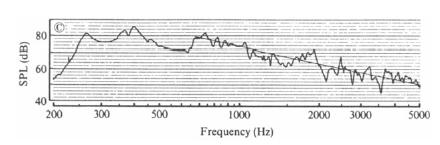
\includegraphics[width=0.9\linewidth]{00_Images/03_chapter/img402.jpg}
\caption{Radiated sound pressure level versus frequency}
\label{fig:violin_spl_spectrum}
\end{figure}

\subsection{Directivity and Frequency Dependence}

A directional analysis of the radiated sound highlights a change of behavior above a characteristic frequency on the order of \SI{1000}{\hertz}. 

\begin{itemize}
    \item Below that frequency, the radiation pattern is smooth and the instrument is approximately omnidirectional, especially below \SI{500}{\hertz}.
    \item Above about \SI{1000}{\hertz}, the instrument becomes progressively more directive.
    \item Near a resonance, small changes in frequency can produce dramatic changes in the radiation pattern.
\end{itemize}

\subsection{Directional Characteristics at Selected Frequencies}

Polar radiation plots measured on different violins driven sinusoidally at the bridge illustrate how the directivity evolves across frequency. Representative patterns reported at frequencies such as \SI{695}{\hertz}, \SI{875}{\hertz}, \SI{625}{\hertz}, and \SI{650}{\hertz} show that even in a relatively narrow band, the radiated field can differ substantially between instruments and between nearby frequencies. Directional characteristics of violin radiation at a representative frequency are shown in figure \ref{fig:violin_directivity_comparison}.

\begin{figure}[!htb]
\centering
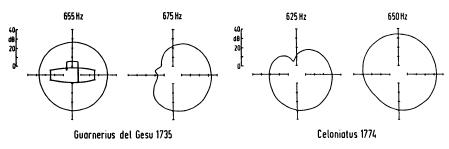
\includegraphics[width=0.8\linewidth]{00_Images/03_chapter/img418.jpg}
\caption{Directional characteristics of radiated sound for two violins}
\label{fig:violin_directivity_comparison}
\end{figure}

\subsection{Principal Radiation Directions}

If directivity characteristics are averaged over wider frequency ranges and over multiple instruments, one obtains a set of principal radiation directions. These can be summarized by showing the angular regions within \SI{3}{\decibel} of the maximum on selected planes, for instance on horizontal and vertical planes for the cello, and on the horizontal plane for the violin. A compact summary of the main radiation directions (in terms of \SI{3}{\decibel} regions) is shown in figure \ref{fig:violin_radiation_3db_regions}.

\begin{figure}[!htb]
\centering
\subfloat{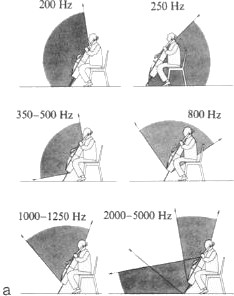
\includegraphics[width=0.3\linewidth]{00_Images/03_chapter/img442_1.jpg}}\hfill
\subfloat{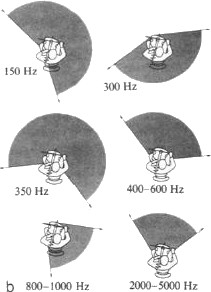
\includegraphics[width=0.3\linewidth]{00_Images/03_chapter/img442_2.jpg}}\hfill
\subfloat{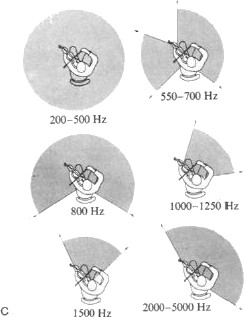
\includegraphics[width=0.3\linewidth]{00_Images/03_chapter/img442_3.jpg}}
\caption{Main radiation directions summarized as \SI{3}{\decibel} regions}
\label{fig:violin_radiation_3db_regions}
\end{figure}
 
\section{The Wolf Notes}

A wolf note is an unstable regime that arises from a strong coupling between the bowed string and a prominent body resonance. An example illustrating the temporal behavior during a wolf note is shown in figure \ref{fig:wolf_note_oscillograms}.

\begin{figure}[!htb]
\centering
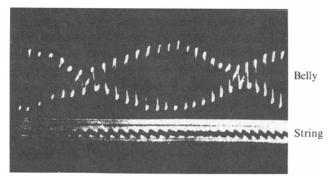
\includegraphics[width=0.7\linewidth]{00_Images/03_chapter/img457.jpg}
\caption{Example oscillograms during a wolf note}
\label{fig:wolf_note_oscillograms}
\end{figure}

\paragraph{Impedance mismatch and cyclic energy transfer} In normal conditions, the characteristic impedance of a string is about \( 1/10 \) of the bridge impedance as seen by the string. This mismatch is usually large enough to treat the bridge as effectively rigid, providing the strong reflection needed for oscillations to build up on the string. At the frequency of a strong body resonance, however, the bridge impedance is greatly reduced. The resulting reflection can become too weak to compensate the losses inherent to the string motion. The interaction can then proceed as follows:

\begin{itemize}
    \item Initially, the bridge still provides a sufficiently strong reflection for the string oscillation to build up.
    \item As the body vibration builds up near the resonance, the bridge appears comparatively soft to the string and absorbs energy, causing the string oscillation to die down.
    \item When the string oscillation weakens, the body vibration is deprived of its energy source and decays as well, enabling the cycle to start again.
\end{itemize}

\paragraph{Amplitude exchange and perceived roughness} The net result is an alternation in which string and body vibrations grow and diminish in amplitude in turn. The perceived tone varies strongly and harshly at an exchange frequency that is typically about \SI{5}{\hertz}.

\paragraph{Why cello and viola are more prone} The instruments most prone to wolf notes are the cello and the viola. Their dimensions are not scaled proportionally to the wavelength of the sounds they produce, so the impedance mismatch between bridge and string is reduced with respect to the violin. In addition, the larger bridge height acts as a longer lever, further reducing the impedance seen by the string. The wolf note is most likely to be triggered under light bowing, because the exerted force may be insufficient to compensate the losses.

\paragraph{Simulation evidence} A simple simulation can reproduce the phenomenon by adding a single body resonance at the same frequency as the fundamental of the string. The time histories show a visible modulation of the string velocity, associated with an alternation between Helmholtz motion and a double-slipping regime. In the simulated behavior, Helmholtz motion breaks down when body motion reaches a high value and resumes when body motion becomes sufficiently small.

\section{Electric Analog of the Violin}

The violin can be interpreted as a broadband radiator obtained by distributing many relatively narrow resonances across frequency, rather than by relying on one or two nearly aperiodic bands. In the upper octaves the wooden body provides a sufficiently dense set of resonances to yield a quasi-uniform response, while in the lower octaves the series ends and a prominent resonance in the vicinity of \SI{460}{\hertz} is often identified as the main body resonance. Without additional reinforcement below this region, the response would tend to decrease rapidly with frequency. The air resonance associated with the cavity breathing through the f-holes supports the response over part of the next octave. A further point is that subjective uniformity is not solely determined by the objective frequency response. A strengthened harmonic can increase the perceived strength of the corresponding fundamental, reducing the perceptual impact of dips in the measured curve and contributing to tone-color differences. An overview of an electrical analog representation of the violin is shown in figure \ref{fig:violin_electric_analog_overview}. 

\begin{figure}[!htb]
\centering
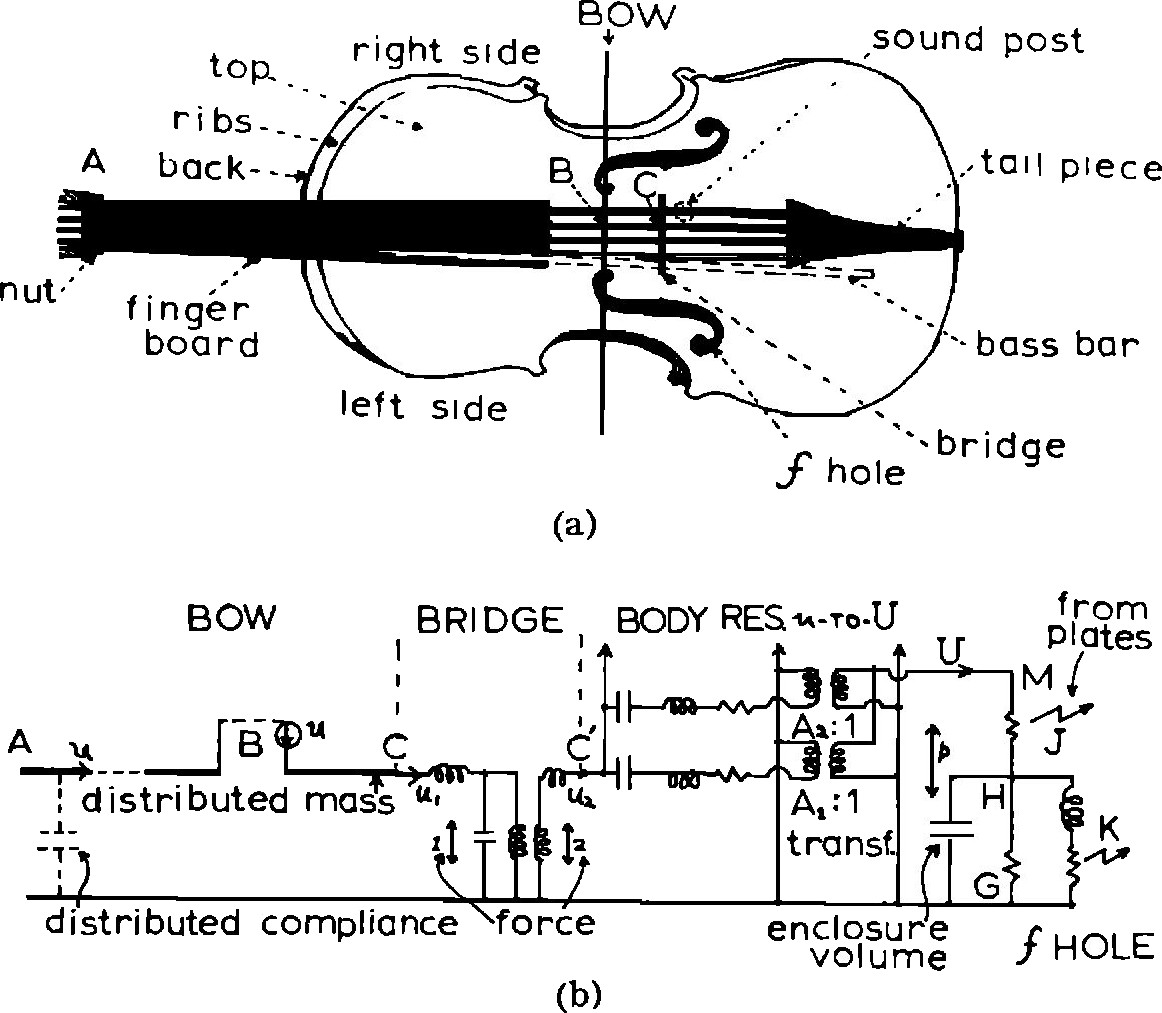
\includegraphics[width=0.7\linewidth]{00_Images/03_chapter/img476.jpg}
\caption{Overview of an electrical analog of the violin}
\label{fig:violin_electric_analog_overview}
\end{figure}

\subsection{String}

In an electrical analogy based on the impedance (force-velocity) convention, the circuit begins at the bow-string contact, which can be represented by a negative resistance. Under the Helmholtz model of bowed-string motion, the bow-string contact behaves as a velocity generator, and the contact point is in series with the two string segments it defines. The two segments have different reactive characters: the segment toward one end can be treated as a positive mechanical reactance, while the other appears as a negative reactance, except as modified by the bridge. Taken together, the two parts form a distributed resonant system. Since the traveling-wave wavelength on the string is comparable with the string length, a transmission-line representation is appropriate.

\subsection{The Bridge}

The bridge is the transducer that accepts power from the string and conveys it to the body, which then excites both the surrounding air and the internal cavity air. Since bridge resonances occur at frequencies high with respect to the lower octaves of the string, the bridge can be regarded as effectively rigid in that range and modeled mainly as a transformer, without introducing a dominant filtering effect there. 

\subsection{The Soundpost}

At low frequencies, the soundpost can be approximated as an element that connects top and back plates together with the ribs. In addition, the soundpost is a main source of asymmetry in mode shapes, which contributes to more efficient radiation than would be expected for a perfectly symmetric structure excited in a purely antisymmetric manner.

\subsection{The Body Modes}

The f-holes, even if narrowed through historical evolution, remain relevant in sound emission, especially for the breathing-type air motion. In the impedance view, the body response exhibits alternating resonances and antiresonances. Due to losses and radiation, resonant impedances do not reach zero. A key observation is that body resonances do not necessarily correspond to maxima in the acoustic response, because many structural modes radiate poorly. Modes with efficient radiation properties play a disproportionate role in the radiated output. In the circuit representation, plate modes can be rendered as a parallel set of resonant branches connected at the bridge coupling point. 

\subsection{The Air Mode}

Air modes represent efficient radiators and form a notable exception to the previous observation. In the circuit, this contribution is described in terms of volume velocity and coupled through a mechanical-to-acoustical transformer with ratio \( A:1 \), where \( A \) depends on the mode considered. The radiation through the f-holes is represented by the branch associated with the apertures. Since the apertures are not circular and the violin walls are not rigid, the resonance frequency is not expected to coincide exactly with the ideal Helmholtz value. Nevertheless, experiments indicate that the deviation remains limited even with non-rigid walls, and it stays small for approximately elliptical apertures with modest eccentricity. 

\subsection{Simplified Circuit: Air Resonance and One Body Resonance}

If only the air resonance and the main body resonance are retained, a simplified network is obtained in which one resonant body branch is combined with the air branch, and the coupling is referred to the bridge. This reduced description is useful to interpret how the lower register can be strengthened by matching the air resonance and the main body resonance, rather than treating them as isolated phenomena.

\subsection{Loss Mechanisms}

Within the simplified circuit, a transient associated with the air branch suffers from losses due to thermal and viscous effects in air, losses within the wood, and radiation losses. It is found that wood-related losses are typically much larger than those associated with air viscosity, so the dominant contributions are radiation and wood losses. As the air volume of the enclosure increases, radiation losses increase while wall-related losses decrease, leading to a trade-off that can be explored by varying geometric parameters. 

\subsection{Rib Height and Loss Balance}

By fixing top and back plates and varying rib height, the combined losses show a minimum at an intermediate rib height. The reported trend indicates that the rib height that minimizes the total losses is close to the rib height found in standard violin construction. 
